\section*{Background}

\subsection*{Neural Radiance Fields}

Neural Radiance Fields (NeRF)~\cite{mildenhall2020nerf} are a recent technique for novel view synthesis. In order to represent a highly-detailed scene, NeRF models a scene as a continuous, volumetric field of varying density, which refracts light at varying degrees. This is based on traditional volumetric rendering techniques, based on the rendering equation:
\[
  I(r) = \int_{t_n}^{t_f} T(t, r) \sigma(r(t)) c(r(t), r_d)dt
\]
Where 
\[
    T(t, r) = \exp{-\int_{t_n}^{t} \sigma(r(s))ds}
\].

Where $I(r)$ is the illumination along camera ray $r(t) = r_o + t r_d$. Neural radiance fields are able to accurately reconstruct high-frequency features by recovering $\sigma$, the density at a given point, and $c$, the view-dependent color at a given point by modelling them as MLPs with an additional encoding scheme that allows for differentiation between extremely close points. We evaluate the above equations by performing ray-marching and computing $T(j,r) = \Sigma -\exp\sigma_i c_i$, by partitioning the ray into evenly spaced bins and sampling randomly from within each bin.

There have been a significant number of extensions to NeRF, including optimizations on the encoding for differentiating positions in space~\cite{tancik2020fourfeat}, better sampling approaches~\cite{barron2021mipnerf}, and faster training~\cite{yu2021plenoxels}. This is only a small subset of NeRF variants, and a plethora exist which we do not list.

\subsection*{Dynamic Neural Radiance Fields}

Neural Radiance Fields were designed to only handle static scenes, and thus cannot accurately reconstruct scenes which contain movement, alternative lighting conditions, or other variations.
In order to model dynamic scenes, there have been two diverging approaches. 

One subset of approaches directly model the transformation in the time domain, by directly modelling the function $\sigma(x,t)=f(x\in\mathbb{R}^3, t\in[0,1])$, which include works such as HyperNeRF~\cite{park2021hypernerf}, NeRFies~\cite{park2021nerfies}, and Space-Time Invariant Irradiance Fields~\cite{xian2021space}. By directly modelling the variation of the density, these methods are able to reconstruct large deformations in latent spaces and reconstruct a wide variety of transformations from a single radiance field, often allowing for transformations in some latent space that permit for deformation.

The other subset of approaches models dynamics directly as a form of translation. In this case, we are not able to directly move the objects inside the scene since we can only evaluate the NeRF at a given $x$, so instead we invert the translation, instead bending the rays as a function of time, which acts to warp the space being rendered. This allows for effective simulation, and can be post-processed to compute object translation if so desired. The formulation for density is thus better described as $\sigma(x,t)=f(x+\Delta(x,t))$. This formulation enforces a coherent canonical representation, while directly modelling movement, and has been shown to be able to reconstruct both synthetic with D-NeRF~\cite{pumarola2020dnerf} and real scenes in NR-NeRF~\cite{tretschk2021nonrigid}.

The pros of directly including time as a function in the MLP are that we are able to represent a much broader class of functions, in theory every frame may be fully distinct from the previous, but the canonical formulation lends itself to smoothness between frames. Our approach falls into the canonization category, since we are interested in accurately reconstructing smooth movement as opposed to generalizing over many classes of movement.

\subsection*{Bezier Curves}

Bezier curves refer to a class of functions defined as a polynomial parametrized by a set of
control points. They are most commonly used as cubic polynomials: $f(x) = ax^3 + bx^2 + cx + d$,
where x is the variable we are interested in interpolating over. The general formulation for
the Bezier basis functions is defined as $B^n(t) = \Sigma^n_{i=0}
{n \choose i} (1-t)^{n-i} t^i$ where n
is the degree of the Bezier polynomial. In order to give control of the Bezier curve, we
introduce "control points", which weighs different points along the curve differently:
$B^n(t) = \Sigma^n_{i=0} P_i {n \choose i} (1-t)^{n-i} t^i$, where $P_i\in\mathbb{R}^3$ for 3D
movement. For a more comprehensive guide on Bezier splines, we refer the reader to a more
\href{https://pomax.github.io/bezierinfo/index.html}{complete reference}.

\begin{figure}
    \centering
    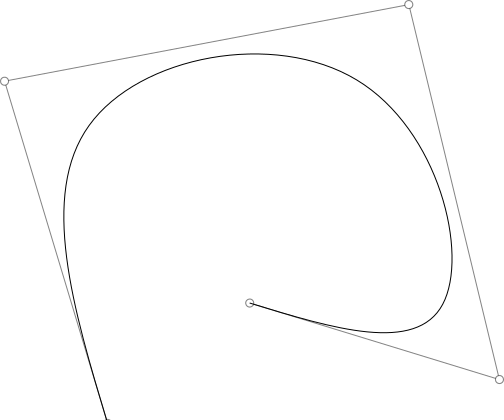
\includegraphics[width=0.5\textwidth]{bezier_curve.png}
    \caption{
        Bezier Curves are a low dimensional representation of smooth interpolation between a few control points. We leverage them to represent smooth movement and produce a prior over movement. Credit to Wikipedia~\cite{bezier_diagram} for diagram.
    }
    \label{fig:my_label}
\end{figure}

